\subsection{First Brocard triangle: vertex locus}

Consider a triangle $T=P_1 P_2  P_3 $ with Brocard points $\Omega_1$ and $\Omega_2$. Referring to Figure~\ref{fig:06-first-broc-tri}:

\begin{definition}[First Brocard Triangle]
The vertices $P_1'$, $P_2'$, $P_3'$ of the First Brocard Triangle $T_1$ are defined as follows: $P_1'$ (resp. $P_2'$, $P_3'$) is the intersection of $P_2{\Omega_1}$ (resp. $P_3{\Omega_1}$, $P_1{\Omega_1}$) with $P_3{\Omega_2}$ (resp. $P_1{\Omega_2}$, $P_2{\Omega_2}$).
\end{definition}

Know properties of the $T_1$ include that (i) it is inversely similar to $T$, (ii) its barycenter $X_2$ coincides with that of the reference triangle, and (iii) its vertices are concyclic with $\Omega_1$, $\Omega_2$, $X_3$, and $X_6$ on the Brocard circle \cite[Brocard Circle]{mw}, whose center is $X_{182}$. Referring to Figure~\ref{fig:06-homot-loci}:

\begin{figure}
    \centering
    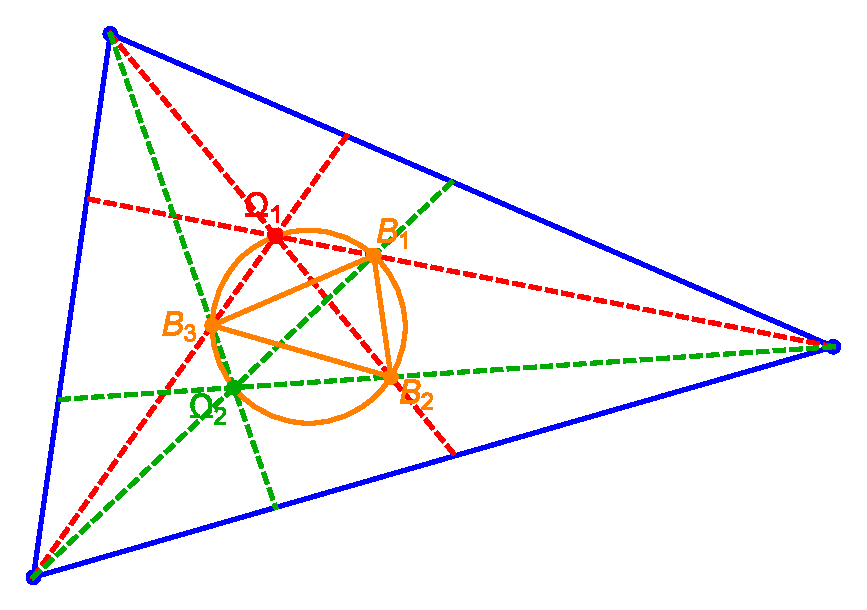
\includegraphics[width=.7\textwidth]{pics_06_070_first_brocard_tri}
    \caption{Construction for the First Brocard Triangle (orange) taken from \cite[First Brocard Triangle]{mw}. It is inversely similar to the reference one (blue), and their barycenters $X_2$ are common. Its vertices $B_1,B_2,B_3$ are concyclic with the Brocard points $\Omega_1$ and $\Omega_2$ on the Brocard circle (orange).}
    \label{fig:06-first-broc-tri}
\end{figure}

\begin{proposition}
Over 3-periodics in the homothetic pair, the locus of the vertices of $T_1$ is an axis-aligned, concentric ellipse, homothetic to the ones in the pair and interior to the caustic. Its axes are given by: 
\[ a'=\frac{a(a^2-b^2)}{2(a^2+b^2)},\;\;\; b'=\frac{b(a^2-b^2)}{2(a^2+b^2)}\]
\end{proposition}

\begin{proof}
The locus must be an ellipse since $T_1$ is inversely similar to the 3-periodics whose vertices are inscribed in an ellipse and their barycenters coincide. A vertex of the Brocard triangle is parametrized by

\[ \frac{x^2}{a'^2}+\frac{y^2}{b'^2} = 1 \]
\end{proof}

Since homothetic 3-periodics conserve area \cite{reznik2020-similarityII}, so must $T_1$ (inversely similar). Its area can be computed explicitly:

\begin{proposition}
Over 3-periodics in the homothetic pair, the area of $T_1$ is invariant and given by
\[ {\frac {3\sqrt{3} ab\left( {a}^{2}-{b}^{2} \right) ^{2}  }{16
 \left( {a}^{2}+{b}^{2} \right) ^{2}}}
\]
\end{proposition}





